% Options for packages loaded elsewhere
\PassOptionsToPackage{unicode}{hyperref}
\PassOptionsToPackage{hyphens}{url}
\PassOptionsToPackage{dvipsnames,svgnames*,x11names*}{xcolor}
%
\documentclass[
  11pt,
]{article}
\usepackage{lmodern}
\usepackage{amssymb,amsmath}
\usepackage{ifxetex,ifluatex}
\ifnum 0\ifxetex 1\fi\ifluatex 1\fi=0 % if pdftex
  \usepackage[T1]{fontenc}
  \usepackage[utf8]{inputenc}
  \usepackage{textcomp} % provide euro and other symbols
\else % if luatex or xetex
  \usepackage{unicode-math}
  \defaultfontfeatures{Scale=MatchLowercase}
  \defaultfontfeatures[\rmfamily]{Ligatures=TeX,Scale=1}
\fi
% Use upquote if available, for straight quotes in verbatim environments
\IfFileExists{upquote.sty}{\usepackage{upquote}}{}
\IfFileExists{microtype.sty}{% use microtype if available
  \usepackage[]{microtype}
  \UseMicrotypeSet[protrusion]{basicmath} % disable protrusion for tt fonts
}{}
\makeatletter
\@ifundefined{KOMAClassName}{% if non-KOMA class
  \IfFileExists{parskip.sty}{%
    \usepackage{parskip}
  }{% else
    \setlength{\parindent}{0pt}
    \setlength{\parskip}{6pt plus 2pt minus 1pt}}
}{% if KOMA class
  \KOMAoptions{parskip=half}}
\makeatother
\usepackage{xcolor}
\IfFileExists{xurl.sty}{\usepackage{xurl}}{} % add URL line breaks if available
\IfFileExists{bookmark.sty}{\usepackage{bookmark}}{
\usepackage{hyperref}
}
\hypersetup{
  pdftitle={Memento ligne de commandes, shell bash},
  pdfauthor={Première NSI, Lycée du Parc},
  colorlinks=true,
  linkcolor=Maroon,
  filecolor=Maroon,
  citecolor=Blue,
  urlcolor=Blue,
  pdfcreator={LaTeX via pandoc}}
\urlstyle{same} % disable monospaced font for URLs
\usepackage[top=20mm,left=20mm,right=20mm,heightrounded]{geometry}
\usepackage{graphicx}
\makeatletter
\def\maxwidth{\ifdim\Gin@nat@width>\linewidth\linewidth\else\Gin@nat@width\fi}
\def\maxheight{\ifdim\Gin@nat@height>\textheight\textheight\else\Gin@nat@height\fi}
\makeatother
% Scale images if necessary, so that they will not overflow the page
% margins by default, and it is still possible to overwrite the defaults
% using explicit options in \includegraphics[width, height, ...]{}
\setkeys{Gin}{width=\maxwidth,height=\maxheight,keepaspectratio}
% Set default figure placement to htbp
\makeatletter
\def\fps@figure{htbp}
\makeatother
\setlength{\emergencystretch}{3em} % prevent overfull lines
\providecommand{\tightlist}{%
  \setlength{\itemsep}{0pt}\setlength{\parskip}{0pt}}
\setcounter{secnumdepth}{5}

\title{Memento ligne de commandes, shell bash}
\usepackage{etoolbox}
\makeatletter
\providecommand{\subtitle}[1]{% add subtitle to \maketitle
  \apptocmd{\@title}{\par {\large #1 \par}}{}{}
}
\makeatother
\subtitle{Thème architectures matérielles et systèmes d'exploitation}
\author{Première NSI, \href{https://frederic-junier.org/}{Lycée du
Parc}}
\date{}

%%%jolis boites

\usepackage{fancybox, graphicx}



%%%%%%%%%%%%%%%%Packages et Macros Frederic%%%%%%%%%%%%%%%%%%%%%%%%%%%%%


%%%%Insertion de liens hypertextes %%%%

            
%%%%%%%%%%PSTricks%%%%%%%%%%%%

\usepackage{pstricks,pst-plot,pst-text,pst-tree,pst-eps,pst-fill,pst-node,pst-math,pstricks-add,pst-xkey,pst-eucl}


%%%%%%%Tikz%%%%%%%%%%%%%%%
\usepackage{pgf,tikz,tkz-tab}
% Pour les tableaux de signes ou de variations avec tkz-tab voir https://zestedesavoir.com/tutoriels/439/des-tableaux-de-variations-et-de-signes-avec-latex/#1-13389_tikz-un-package-qui-en-a-dans-le-ventre
\usetikzlibrary{arrows}
\usetikzlibrary{shapes.geometric}
\usetikzlibrary{shapes.geometric}
\usetikzlibrary{petri}
\usetikzlibrary{decorations}
\usetikzlibrary{arrows}
\usetikzlibrary{math}
 %Variables must be declared in a tikzmath environment but
       % can be used outside
%       \tikzmath{int \n; \n = 508; \x1 = 1; \y1 =1; 
%                   %computations are also possible
%                    \x2 = \x1 + 1; \y2 =\y1 +3; } 


%%%%%%%%%%%%%%%%%%%%%%%%%%%%%%%%%%%%%%%%
%%%%%%%%%%%Commandes Tikz Perso%%%%%%%%%%%%%%%

% Définition des nouvelles options xmin, xmax, ymin, ymax
% Valeurs par défaut : -3, 3, -3, 3
\tikzset{
xmin/.store in=\xmin, xmin/.default=-3, xmin=-3,
xmax/.store in=\xmax, xmax/.default=3, xmax=3,
ymin/.store in=\ymin, ymin/.default=-3, ymin=-3,
ymax/.store in=\ymax, ymax/.default=3, ymax=3,
}
% Commande qui trace la grille entre (xmin,ymin) et (xmax,ymax)
\newcommand {\grille}[2]
{\draw[help lines,black, thick] (\xmin,\ymin) grid[xstep=#1, ystep=#2] (\xmax,\ymax);}
% Commande \axes
\newcommand {\axes} {
\draw[->,very thick] (\xmin,0) -- (\xmax,0);
\draw[->,very thick] (0,\ymin) -- (0,\ymax);
\draw (0.95*\xmax, 0) node[above] {};
\draw (0, 0.95*\ymax) node[left] {};
}
% Commande qui limite l?affichage à (xmin,ymin) et (xmax,ymax)
\newcommand {\fenetre}
{\clip (\xmin,\ymin) rectangle (\xmax,\ymax);}

%Exemple d'utilisation

%\begin{center}
%\begin{tikzpicture} [xmin=-2,xmax=2,ymin=0,ymax=5]
%\grille{1} \axes \fenetre
%\draw plot[smooth] (\x,\x^2);
%\end{tikzpicture}
%\end{center}

%style pour la perspective cavalière française
%voir Tikz pour l'impatient page 68
\tikzset{math3d/.style=
{x= {(-0.353cm,-0.353cm)}, z={(0cm,1cm)},y={(1cm,0cm)}}}

%%%%%%%Symbole pour code calculatrice%%%%%%

%Flèche remplie pour défilement de menu

\newcommand{\flechefillright}{

\begin{tikzpicture}[scale=0.15] \fill (0,0)--(2,1)--(0,2)--cycle;
\end{tikzpicture}}

%%%%%%%%%%%%%Symboles pour calculatrice Casio%%%%
\newcommand{\execasio}{\Pisymbol{psy}{191}} %Retour chariot
\newcommand{\dispcasio}{\begin{pspicture}(.1,.1)\pspolygon*(.1,0)(.1,.1)\end{pspicture}} %Triangle « Disp »
\newcommand{\dispcasiotikz}{
\begin{tikzpicture}[scale=0.2]
\fill (0,0) -- (1,0) -- (1,1) -- cycle;
\end{tikzpicture}} %Triangle « Disp »
%

%Fleche entre deux lignes, d'apres 'un bon petit' : http://forum.mathematex.net/latex-f6/fleches-entre-deux-lignes-pour-resolution-d-equation-t10283.html#p99817
\newcommand\addnode[1]{\Rnode{#1}{}}
\newcommand\linknode[3]{\ncbar[angleA=0,angleB=0,nodesep=1ex,arm=10ex,offset=-2pt]{->}{#1}{#2}\Aput{\vphantom{x}#3}}


%%Commande pour touche de calculatrice

\newcommand\tc[1]{%
{
\begin{tikzpicture}
\node[draw,rectangle,rounded corners=3pt] (P) at (0,0){#1};
\end{tikzpicture}
}
}

%%%%%%%%%%%%%%%%%%%%%%%%%%%%%%%%%%%%%%%%
%%%%%%%%%%%Fin Commandes Tikz%%%%%%%%%%%%%%%


%%%%%%%%%%%%Specifiques%%%%%%%%%%%
\usepackage{wrapfig}
%pour insérer une figure à droite ou à gauche d'un texte
%\begin{wrapfigure}[nb lignes]{placement l,r,c,i(inside),o(outside)}[overhang]{width}
%ce package fonctionne mal à proximité des listes
%%%%%%%%%%%%%%%%%%%%%%%%%%%%%%%%%%%%%

%%%%%Environnements et symboles spéciaux pour faire joli%%%%%%

%%%Bclogo, pour des environnements + jolis avec insertion de logo%%%%
%Dépendances de  bclogo
\usepackage{xkeyval}  
\usepackage{etoolbox}
\usepackage{ifpdf}
\usepackage[framemethod=tikz]{mdframed}
\usepackage[tikz]{bclogo}

%\newcommand\bcpython{\includegraphics[width=17pt]{/home/fjunier/Maths/python-logo.eps}}
\newcommand\bcpython{\includegraphics[width=17pt]{/home/fjunier/Maths/python-logo.png}}
%\newcommand\bcpython{\includegraphics[width=17pt]{/home/frederic/Maths/python-logo.png}}

%% Framed
\usepackage{framed}  %Le package « framed» Crée 3 nouveaux environnements, qui se comportent comme des minipage de largeur \linewidth, mais permettant en plus de se casser entre plusieurs pages.     * framed : avec un cadre autour;     * shaded : avec un fonc coloré (il faut définir la couleur shadecolor);     * leftbar : avec une barre le long du côté gauche.

%%%%%%%%%%%%%%%%%%%Présentation de codes sources%%%%%%%%%%%%%%%%%
\usepackage{listings}
%On utilise l?environnement lstlisting pour insérer
%un code source.
%En plus de l?environnement lstlisting, on peut également utiliser la
%commande \lstinline qui fonctionne comme la commande \verb, en ce
%sens qu?on peut utiliser n?importe quel caractère comme délimiteur. Enfin,
%la commande \lstinputlisting permet de charger un code source depuis
%un fichier externe.
%Il y a deux manières de préciser des options : soit via l?option de l?envi-
%ronnement ou de la commande, soit en utilisant la commande \lstset
%qui permet de définir des options de manière globale.

\lstset{ %
  language=Python,                % the language of the code
  basicstyle=\ttfamily,           % the size of the fonts that are used for the code
  %numbers=left,                   % where to put the line-numbers
  numberstyle=\tiny,  % the style that is used for the line-numbers
  %stepnumber=2,                   % the step between two line-numbers. If it's 1, each line 
                                  % will be numbered
  %numbersep=5pt,                  % how far the line-numbers are from the code
  backgroundcolor=\color{white},      % choose the background color. You must add \usepackage{color}
  showspaces=false,               % show spaces adding particular underscores
  showstringspaces=false,         % underline spaces within strings
  showtabs=false,                 % show tabs within strings adding particular underscores
  frame=single,                   % adds a frame around the code
  rulecolor=\color{black},        % if not set, the frame-color may be changed on line-breaks within not-black text (e.g. comments (green here))
  tabsize=4,                      % sets default tabsize to 2 spaces
  captionpos=b,                   % sets the caption-position to bottom
  breaklines=true,                % sets automatic line breaking
  breakatwhitespace=false,        % sets if automatic breaks should only happen at whitespace
  %title=\lstname,                   % show the filename of files included with \lstinputlisting;
                                  % also try caption instead of title
  breakindent=1cm,
  keywordstyle=\color{blue},          % keyword style
  commentstyle=\color{red},       % comment style
  %stringstyle=\ttfamily\color{green},         % string literal style
  escapeinside={\%*}{*)},            % if you want to add LaTeX within your code
  morekeywords={*,...},              % if you want to add more keywords to the set
  deletekeywords={...}              % if you want to delete keywords from the given language
  upquote=true,columns=flexible,
xleftmargin=1cm,xrightmargin=1cm,
 inputencoding=utf8,			%Les lignes qui suivent sont pour le codage utf8
  extendedchars=true,
  literate=%
            {é}{{\'{e}}}1
            {è}{{\`{e}}}1
            {ê}{{\^{e}}}1
            {ë}{{\¨{e}}}1
            {û}{{\^{u}}}1
            {ù}{{\`{u}}}1
            {â}{{\^{a}}}1
            {à}{{\`{a} }}1
            {î}{{\^{i}}}1
            {ô}{{\^{o}}}1
            {ç}{{\c{c}}}1
            {Ç}{{\c{C}}}1
            {É}{{\'{E}}}1
            {Ê}{{\^{E}}}1
            {À}{{\`{A}}}1
            {Â}{{\^{A}}}1
            {Î}{{\^{I}}}1
}

\lstdefinestyle{rond}{
  numbers=none,
  backgroundcolor=\color{gristclair},
  frameround =tttt
}

\lstdefinestyle{compil}{
  numbers=none,
  backgroundcolor=\color{gristclair}
}
%\lstset{language=Python,basicstyle=\small , frame=single,tabsize=4,showspaces=false,showtabs=false,showstringspaces=false,numbers=left,numberstyle=\tiny , extendedchars=true}



%%%%%%%%%%%%%%%%%%%%%%%%%%%%%%%%%%%%%%%%%%%%%%%%%%%%%%%%%%%%%%%%%%%%%%%%
%%%%%%%%%%%%%%%%%%%%Environnements persos%%%%%%%%%%%%%%%%%%%%%%%%%%%%%%%%
%Syntaxe :
%\newenvironment{nom}[nombre d'args][defaut]{definitions initiales}{definitions finales}
%definitions intiales sont les commandes appelées par \begin{nom}
%Definitions finales sont les commandes appelées par \end{nom}

%%%%%%%%%%%%%%%%Définitions des environnemts persostheoreme, exemple ..%%%%
%%%% Exercice avec encadré %%%%
\newcounter{exo}
\newenvironment{exercice}[1]
{\par \medskip   \addtocounter{exo}{1} \noindent  
\begin{bclogo}[arrondi =0.1,   noborder = true, logo=\bccrayon, marge=4]{~\textbf{Exercice} \textbf{\theexo} {\itshape #1} }  \par}
{
\end{bclogo}
 \par \bigskip }

%%Axiomes, Theoremes, Propriété, Définition, Methode, Preuve


\newenvironment{axiome}[1]
{\par \medskip   \begin{leftbar} \noindent \underline{\textbf{Axiome}}\hspace{0.5cm}{\itshape #1}   \vspace*{10pt} \par }
{\end{leftbar}  \par \medskip }


\newcounter{thme}
\newenvironment{theoreme}[1]
{\par \medskip  \addtocounter{thme}{1} \noindent  
\begin{bclogo}[arrondi =0.1,  ombre = true, barre=none, logo=\bcbook, marge=4]{~\textbf{Théorème} \textbf{\thethme} {\itshape #1} }   \par}
{
\end{bclogo}
 \par \bigskip}

 \newenvironment{theoremedef}[1]
{\par \medskip   \addtocounter{thme}{1} \noindent  
\begin{bclogo}[arrondi =0.1,  ombre = true, barre=none, logo=\bcbook, marge=4]{~\textbf{Théorème-Définition} \textbf{\thethme} {\itshape #1} }   \par}
{
\end{bclogo}
 \par \bigskip }
 
\newcounter{prop}
\newenvironment{propriete}[1]
{\par \medskip   \addtocounter{prop}{1} \noindent  
\begin{bclogo}[arrondi =0.1,  ombre = true, barre=none, logo=\bcbook, marge=4]{~\textbf{Propriété} \textbf{\theprop} {\itshape #1} }   \par}
{
\end{bclogo}
 \par \bigskip }


\newenvironment{corollaire}[1]
{\par \medskip   \noindent  
\begin{bclogo}[arrondi =0.1,  ombre = true, barre=none, logo=\bcbook, marge=4]{~\textbf{Corollaire} {\itshape #1} } \par }
{
\end{bclogo}
 \par \bigskip }

\newenvironment{demo}[1]
{\par \medskip   \noindent  
\begin{bclogo}[arrondi =0.1,  ombre = true, barre=zigzag, noborder = true, logo=\bcloupe, marge=0]{~\textbf{Démonstration} {\itshape #1} } \par \vspace{10pt}}
{
\end{bclogo}
 \par \bigskip }

\newcounter{activite}
\newenvironment{activite}[1]
{\par \medskip   \noindent   \addtocounter{activite}{1}
\begin{bclogo}[arrondi =0.1,   noborder = true, logo=\bcvelo, marge=4]{~\textbf{Activité} \textbf{\theactivite} {\itshape #1} }  \par}
{
\end{bclogo}
 \par \bigskip }


\newcounter{rque}
\newenvironment{remarque}
{\par \medskip    \addtocounter{rque}{1} \noindent  
\begin{bclogo}[arrondi =0.1,  ombre = true, barre=snake, noborder = true, logo=\bcinfo, marge=0]{~\textbf{Remarque} \textbf{\therque}}  \par }
{
\end{bclogo}
 \par \bigskip }

\newcounter{def}
\newenvironment{definition}[1]
{\par \medskip   \addtocounter{def}{1} \noindent  
\begin{bclogo}[arrondi =0.1,  ombre = true, barre=none, logo=\bcbook, marge=4]{~\textbf{Définition} \textbf{\thedef} {\itshape #1} }  \par}
{
\end{bclogo}
 \par \bigskip }
 
 
 \newcounter{cours}
\newenvironment{cours}[1]
{\par \medskip   \addtocounter{cours}{1} \noindent  
\begin{bclogo}[arrondi =0.1,  ombre = true, barre=none, logo=\bcbook, marge=4]{~\textbf{Point de cours} \textbf{\thecours} {\itshape #1} }  \par}
{
\end{bclogo}
 \par \bigskip }
 
 

\newenvironment{introduction}
{\par \medskip    \noindent  
 \begin {bclogo}[couleur = blue!5 , arrondi =0.1,logo=\bcrosevents, marge=4] {~\textbf{Introduction}    }
 \par }
{
\end{bclogo}
 \par \bigskip }
 
\newenvironment{memo}[1]
{\par \medskip    \noindent  
\begin{bclogo}[arrondi =0.1,  ombre = true, barre=none, logo=\bccle, marge=4]{~\textbf{À retenir}  {\itshape #1} }  \par}
{
\end{bclogo}
 \par \bigskip }
 
\newcounter{exple}
\newenvironment{exemple}[1]
{\par \medskip   \addtocounter{exple}{1} \noindent  
\begin{bclogo}[arrondi =0.1,   noborder = true, logo=\bclampe, marge=4]{~\textbf{Exemple} \textbf{\theexple} {\itshape #1} }  \par}
{
\end{bclogo}
 \par \bigskip }




\newcounter{alg}
\newenvironment{algorithme}[1]
{\par \medskip   \addtocounter{alg}{1} \noindent  
 \begin {bclogo}[noborder = true, barre=zigzag,logo=\bcpython, marge=4] {~\textbf{Algorithmique} \textbf{\thealg} {\itshape #1} }  \par}
{
\end{bclogo}
 \par \bigskip }

\newcounter{prog}
\newenvironment{programme}[1]
{\par \medskip   \addtocounter{prog}{1} \noindent  
 \begin {bclogo}[noborder = true, barre=zigzag,logo=\bcpython, marge=4] {~\textbf{Programme} \textbf{\theprog} {\itshape #1} }  \par  \bigskip}
{
\end{bclogo}
 \par \bigskip }
 
\newcounter{logi}
\newenvironment{logique}[1]
{\par \medskip   \addtocounter{logi}{1} \noindent  
 \begin {bclogo}[noborder = true, barre=zigzag,logo=\bclampe, marge=4] {~\textbf{Logique} \textbf{\thelogi} {\itshape #1} }  \par}
{
\end{bclogo}
 \par \bigskip }


\newenvironment{methode}[1]
{\par \medskip    \noindent  
 \begin {bclogo}[arrondi =0.1,logo=\bcoutil, marge=4,noborder = true] {~\textbf{Méthode}   {\itshape #1} }  \par}
{
\end{bclogo}
 \par \bigskip }


\newcounter{histo}
\newenvironment{histoire}[1]
{\par \medskip   \addtocounter{histo}{1} \noindent  
 \begin {bclogo}[couleur = blue!10 , arrondi =0.1,logo=\bchorloge, marge=4] {~\textbf{Histoire} \textbf{\thehisto} {\itshape #1} }  \par}
{
\end{bclogo}
 \par \bigskip }




%Environnement contenu pour un document présentant une progression annuelle
\newenvironment{contenu}
{\par \medskip   \begin {bclogo}[ noborder = true,logo=\bccrayon] \noindent {\large \textbf{Contenu de la séance}} \vspace*{10pt} \par  }
{\end{bclogo}  \par \medskip }

%Environnement programme pour un document présentant une progression annuelle
%\newenvironment{programme}
%{\par \medskip   \begin {bclogo}[ noborder = true, barre=zigzag,logo=\bcinfo] \noindent {\large \textbf{Programme officiel}} \vspace*{10pt} \par  }
%{\end{bclogo}  \par \medskip }

%Environnement programme pour un document présentant une progression annuelle
\newenvironment{ressource}
{\par \medskip   \begin {bclogo}[ noborder = true,logo=\bcbook] \noindent {\large \textbf{Ressources}}\\vspace*{10pt} \par }
{\end{bclogo}  \par \medskip }




%%%%%%%%%%%%%%%%%%Maths divers%%%%%%%%%%%%%%%%%%%%%%%%%
%%%%%%%%%%%%%Nombres%%%%%%%%%%%%%%%%

%Ensemble prive de...
%\newcommand{\prive}{\boi}%{\backslash}

%Ensembles de nombres%%%%%%%%%%%%%%%%%
\newcommand{\R}{\mathbb{R}}
\newcommand{\N}{\mathbb{N}}
\newcommand{\D}{\mathbb{D}}
\newcommand{\Z}{\mathbb{Z}}
\newcommand{\Q}{\mathbb{Q}}
%\newcommand{\C}{\mathbb{C}}
\newcommand{\df}{~\ensuremath{]0;+\infty[}~}
\newcommand{\K}{\mathbb{K}}

%%%%%%%%Arithmetique%%%%%%%%%%
%PGCD, PPCM
\newcommand{\PGCD}{\mathop{\rm PGCD}\nolimits}
\newcommand{\PPCM}{\mathop{\rm PPCM}\nolimits}

%Intervalles
\newcommand{\interoo}[2]{]#1\, ;\, #2[}
\newcommand{\Interoo}[2]{\left]#1\, ;\, #2\right[}
\newcommand{\interof}[2]{]#1\, ;\, #2]}
\newcommand{\Interof}[2]{\left]#1\, ;\, #2\right]}
\newcommand{\interfo}[2]{[#1\, ;\, #2[}
\newcommand{\Interfo}[2]{\left[#1\, ;\, #2\right[}
\newcommand{\interff}[2]{[#1\, ;\, #2]}
\newcommand{\Interff}[2]{\left[#1\, ;\, #2\right]}
%\newcommand\interentiers #1#2{[\! [#1\, ;\, #2]\! ]}
\newcommand{\interentiers}[2]{\llbracket #1\, ;\, #2\rrbracket}
%


%%%%%%%%%%%%%%Nombres complexes%%%%%

\newcommand{\ic}{\text{i}}
%\newcommand{\I}{\text{i}}
\newcommand{\im}[1]{\text{Im}\left(#1\right)}
\newcommand{\re}[1]{\text{Re}\left(#1\right)}
\newcommand{\Arg}[1]{\text{arg}\left(#1\right)}
\newcommand{\Mod}[1]{\left[#1\right]}
%Parties entière, réelle, imaginaire, nombre i
\newcommand{\ent}[1]{\text{E}\left(#1\right)}
\renewcommand{\Re}{\mathop{\rm Re}\nolimits}
\renewcommand{\Im}{\mathop{\rm Im}\nolimits}
\renewcommand{\i}{\textrm{i}}

%%%%%%%%%%%Probabilites et statistiques%%%%%
\newcommand{\loibinom}[2]{\mathcal{B}\left(#1\ ; \ #2 \right)}
\newcommand{\loinorm}[2]{\mathcal{N}\left(#1\ ; \ #2 \right)}
\newcommand{\loiexp}[1]{\mathcal{E}\left(#1\right)}
\newcommand{\proba}[1]{\mathbb{P}\big(#1\big)}
\newcommand{\probacond}[2]{\mathbb{P}_{#2}\big(#1\big)}
\newcommand{\esperance}[1]{\mathbb{E}\left(#1\right)}
\newcommand{\variance}[1]{\mathbb{V}\left(#1\right)}
\newcommand{\ecart}[1]{\sigma\left(#1\right)}
\newcommand{\dnormx}{\frac{1}{\sqrt{2\pi}} \text{e}^{-\frac{x^2}{2}}}
\newcommand{\dnormt}{\frac{1}{\sqrt{2\pi}} \text{e}^{-\frac{t^2}{2}}}

%Covariance
\newcommand{\cov}{\mathop{\rm cov}\nolimits}
%


%%%%%%%%%%Analyse%%%%%%%%%%%

%%%%%%%%%%%Courbe%%%%%%%%%%%%
\newcommand{\courbe}[1]{\ensuremath{\mathcal{C}_{#1}}}

%%%%%%%Fonction exponentielle%%%%%
\newcommand{\fe}{~fonction exponentielle~}
\newcommand{\e}{\text{e}}

%Fonction cotangente
\newcommand{\cotan}{\mathop{\rm cotan}\nolimits}
%%%%%%%%%%%%%%%%%%%%%%%%%%%%%%%%%%%%%%%%%
%
%Fonctions hyperboliques
\newcommand{\ch}{\mathop{\rm ch}\nolimits}
\newcommand{\sh}{\mathop{\rm sh}\nolimits}


%%%%%%%%%%%%%%Limites%%%%%%
\newcommand{\limite}[2]{\lim\limits
_{x \to #1} #2}
\newcommand{\limitesuite}[1]{\lim\limits
_{n \to +\infty} #1}
\newcommand{\limiteg}[2]{\lim\limits
_{\substack{x \to #1 \\ x < #1 }} #2}
\newcommand{\limited}[2]{\lim\limits
_{\substack{x \to #1 \\ x > #1 }} #2}

%%%%%%%%%%Continuité%%%%%%%%%%%
\newcommand{\TVI}{théorème des valeurs intermédiaires}

%%%%%%%%%%%Suites%%%%%%%%%%%%
\newcommand{\suite}[1]{\ensuremath{\left(#1_{n}\right)}}
\newcommand{\Suite}[2]{\ensuremath{\left(#1\right)_{#2}}}
%

%%%%%%%%%%%%%%%Calcul intégral%%%%%%
\newcommand{\dx}{\ensuremath{\text{d}x}}		% dx
\newcommand{\dt}{\ensuremath{\text{d}t}}		% dt
\newcommand{\dtheta}{\ensuremath{\text{d}\theta}}		% dtheta
\newcommand{\dy}{\ensuremath{\text{d}y}}		% dy
\newcommand{\dq}{\ensuremath{\text{d}q}}		% dq

%%%Intégrale%%%
\newcommand{\integralex}[3]{\int_{#1}^{#2} #3 \ \dx}
\newcommand{\integralet}[3]{\int_{#1}^{#2} #3 \ \dt}
\newcommand{\integraletheta}[3]{\int_{#1}^{#2} #3 \ \dtheta}

%%%%%Equivalent%%
\newcommand{\equivalent}[1]{\build\sim_{#1}^{}}

%o et O%%%%
\renewcommand{\o}[2]{\build o_{#1\to #2}^{}}
\renewcommand{\O}[2]{\build O_{#1\to #2}^{}}



%%%%%%%%%%%%%%%Geometrie%%%%%%%%%%%%%%%%%%%%%%%

%%%%%%%%%%%%%%%Reperes%%%%%%%%%%%%%%
\def\Oij{\ensuremath{\left(\text{O},~\vect{\imath},~\vect{\jmath}\right)}}
\def\Oijk{\ensuremath{\left(\text{O},~\vect{\imath},~ \vect{\jmath},~ \vect{k}\right)}}
\def\Ouv{\ensuremath{\left(\text{O},~\vect{u},~\vect{v}\right)}}
\renewcommand{\ij}{(\vec\imath\, ;\vec\jmath\,)}
\newcommand{\ijk}{(\vec\imath\, ;\vec\jmath\, ;\vec k\,)}
\newcommand{\OIJ}{(O\,;\, I\,;\, J\,)}
\newcommand{\repere}[3]{\big(#1\, ;\,\vect{#2} ;\vect{#3}\big)}
\newcommand{\reperesp}[4]{\big(#1\, ;\,\vect{#2} ;\vect{#3} ;\vect{#4}\big)}

%%%%%%%%%Coordonnees%%%%%%%%%%%%%%
\newcommand{\coord}[2]{(#1\, ;\, #2)}
\newcommand{\bigcoord}[2]{\big(#1\, ;\, #2\big)}
\newcommand{\Coord}[2]{\left(#1\, ;\, #2\right)}
\newcommand{\coordesp}[3]{(#1\, ;\, #2\, ;\, #3)}
\newcommand{\bigcoordesp}[3]{\big(#1\, ;\, #2\, ;\, #3\big)}
\newcommand{\Coordesp}[3]{\left(#1\, ;\, #2\, ;\, #3\right)}
\newcommand{\Vcoord}[3]{\begin{pmatrix} #1 \\ #2 \\ #3 \end{pmatrix}}
%Symboles entre droites
%\newcommand{\paral}{\sslash}
\newcommand{\paral}{\mathop{/\!\! /}}
%

%%%%%%%%%Produit scalaire, Angles%%%%%%%%%%
\newcommand{\scal}[2]{\vect{#1} \, \cdot \, \vect{#2}}
\newcommand{\Angle}[2]{\left(\vect{#1} \, , \, \vect{#2}\right)}
\newcommand{\Anglegeo}[2]{\left(\widehat{\vect{#1} \, ; \, \vect{#2}}\right)}
\renewcommand{\angle}[1]{\widehat{#1}}
\newcommand{\anglevec}[2]{\left(\vect {#1}\, ,\,\vect {#2} \right)}
\newcommand{\anglevecteur}[2]{(#1\, , \, #2)}
\newcommand{\Anglevec}[2]{(\vecteur{#1}\, ,\,\vecteur{#2})}
\newcommand{\prodscal}[2]{#1 \, \cdot \, #2}
%


%Arc
%\newcommand{\arc}[1]{\wideparen{#1}}
\newcommand{\arcoriente}[1]{\overset{\curvearrowright}{#1}}
%
%


%%%%%%%%%%%%%%%Normes%%%%%%%%%%%%%%%%
\newcommand{\norme}[1]{\left\| #1\right\|}
\newcommand{\normebis}[1]{\delim{2pt}{\|}{9pt}\! #1\delim{2pt}{\|}{9pt}}
\newcommand{\normetriple}[1]{\left |\kern -.07em\left\| #1\right |\kern -.07em\right\|}
\newcommand{\valabs}[1]{\big| \, #1 \, \big|}
%

%%%%%%%%%%%%%%%%%%%%%%%%%%%Degré%%%%%%
%\newcommand{\Degre}{\ensuremath{^\circ}}
%La commande \degre est déjà définie dans le package babel

%%%%%%%%%%Vecteurs%%%%%%%%%%%
\newcommand{\vect}[1]{\mathchoice%
{\overrightarrow{\displaystyle\mathstrut#1\,\,}}%
{\overrightarrow{\textstyle\mathstrut#1\,\,}}%
{\overrightarrow{\scriptstyle\mathstrut#1\,\,}}%
{\overrightarrow{\scriptscriptstyle\mathstrut#1\,\,}}}



%%%%%%%%%%%%%Algebre%%%%%%%%%%%%%%%


%%%%%%%%%%Systemes%%%%%%%%%%%
%Systemes
\newcommand{\sys}[2]{
\left\lbrace
 \begin{array}{l}
  \negthickspace\negthickspace #1\\
  \negthickspace\negthickspace #2\\
 \end{array}
\right.\negthickspace\negthickspace}
\newcommand{\Sys}[3]{
\left\lbrace
 \begin{array}{l}
  #1\\
  #2\\
  #3\\
 \end{array}
\right.}
\newcommand{\Sysq}[4]{
\left\lbrace
 \begin{array}{l}
  #1\\
  #2\\
  #3\\
  #4\\
 \end{array}
\right.}
%
%

%%%%%%%%%%%%%%%%Matrices%%%%%%%%%%%%%%%%%%
%Comatrice
\newcommand{\com}{\mathop{\rm com}\nolimits}
%
%
%Trace
\newcommand{\tr}{\mathop{\rm tr}\nolimits}
%
%
%Transposee
\newcommand{\transposee}[1]{{\vphantom{#1}}^t\negmedspace #1}
%
%
%Noyau
\newcommand{\Ker}{\mathop{\rm Ker}\nolimits}
%
%

%
%Matrices
\newcommand{\Mn}{\mathcal M_n}
\newcommand{\matrice}[4]{
\left(
 \begin{array}{cc}
  #1 & #2 \\
  #3 & #4
 \end{array}
\right)}

\newcommand{\Matrice}[9]{
\left(
 \begin{array}{ccc}
  #1 & #2 & #3\\
  #4 & #5 & #6\\
  #7 & #8 & #9
 \end{array}
\right)}
\newcommand{\Vect}[3]{
\left(\negmedspace
 \begin{array}{c}
  #1\\
  #2\\
  #3
 \end{array}\negmedspace
\right)}
\newcommand{\Ideux}{\matrice{1}{0}{0}{1}}
\newcommand{\Itrois}{\Matrice{1}{0}{0}{0}{1}{0}{0}{0}{1}}
%
%
%Determinants
\newcommand{\determinant}[4]{
\left|
 \begin{array}{cc}
  #1 & #2 \\
  #3 & #4
 \end{array}
\right|}
\newcommand{\Determinant}[9]{
\left|
 \begin{array}{ccc}
  #1 & #2 & #3\\
  #4 & #5 & #6\\
  #7 & #8 & #9
 \end{array}
\right|}

\begin{document}
\maketitle

\renewcommand*\contentsname{Table des matières}
{
\hypersetup{linkcolor=}
\setcounter{tocdepth}{3}
\tableofcontents
}
\hypertarget{cruxe9dits}{%
\section*{Crédits}\label{cruxe9dits}}
\addcontentsline{toc}{section}{Crédits}

\emph{Memento directement inspiré des livres
\href{https://www.eyrolles.com/Informatique/Livre/la-ligne-de-commande-par-l-exemple-9782351410721/}{La
ligne de commande par l'exemple} de Vincent Fourmond et
\href{https://www.eyrolles.com/Informatique/Livre/parlez-vous-shell--9782729877590/}{Parlez-vous
Shell ?} de Thomas Hugel.}

Dans ce memento, nous présentons des commandes du \emph{shell}
\href{https://fr.wikipedia.org/wiki/Bourne-Again_shell}{BASH} sous
licence libre, qui est le \emph{shell} par défaut sur la plupart des
distributions du système d'exploitation libre
\href{https://fr.wikipedia.org/wiki/Linux}{Linux}. On distinguera
parfois fichiers et répertoires mais on rappelle que les répertoires
sont juste des fichiers spéciaux, qui contiennent d'autres fichiers. Un
memento en ligne est disponible sur
\url{https://juliend.github.io/linux-cheatsheet/}.

\emph{Conseils pratiques :} pour faciliter la saisie des commandes avec
le clavier,
\href{https://fr.wikipedia.org/wiki/Bourne-Again_shell}{BASH} offre
quelques raccourcis clavier bien pratiques :

\begin{itemize}
\item
  la touche de tabulation permet d'appeler la complétion automatique qui
  propose de compléter la commande avec les choix possibles (fichiers ou
  commandes existants). Par exemple si on saisit \texttt{pw}, l'appui
  sur la touche de tabulation nous propose plusieurs commandes
  commençant par ce préfixe :

\begin{verbatim}
 junier@fredportable:~$ pw
 pwck      pwconv    pwd       pwdx      pwgen     pwunconv 
\end{verbatim}
\item
  les flèches de direction Haut et Bas permettent de naviguer dans
  l'historique des commandes.
\item
  la plupart des commandes du \emph{shell} sont dotées d'une
  documentation accessible depuis l'interpréteur avec la commande
  \texttt{man}. Par exemple pour afficher l'aide de la commande
  \texttt{ls}, on écrira \texttt{man\ ls}.
\end{itemize}

\hypertarget{un-premier-exemple-de-commande}{%
\section{Un premier exemple de
commande}\label{un-premier-exemple-de-commande}}

Une commande \emph{shell} est constituée du nom de la commande suivi
d'un ou plusieurs arguments. Des options précédées peuvent modifier le
comportement de la commande :

\begin{verbatim}
nom_commande -option1 -option2 ... arg1 arg2 arg3 ... 
\end{verbatim}

Ainsi, la commande \texttt{ls} permet d'afficher des informations sur
répertoire ou un fichier :

\begin{itemize}
\item
  Sans argument, ni option \texttt{ls} liste le contenu du répertoire
  courant :

\begin{verbatim}
  junier@fredportable:~/sandbox$ ls
  fichier1  fichier2  fichier3  fichier4  rep1  rep2  
\end{verbatim}
\item
  Avec l'option \texttt{-l} elle affiche des informations détaillées sur
  chacun des fichiers contenus dans le répertoire :

\begin{verbatim}
  junier@fredportable:~/sandbox$ ls -l
  total 8
  -rw-rw-r-- 1 junier junier    0 août  16 21:43 fichier1
  ...........
  drwxrwxr-x 2 junier junier 4096 août  16 21:44 rep1
  drwxrwxr-x 2 junier junier 4096 août  16 21:44 rep2
\end{verbatim}
\item
  L'option \texttt{-a} affiche les fichiers (ou répertoires cachés) et
  l'option \texttt{-h} convertit les tailles de fichiers (en octets par
  défaut) en des multiples plus lisibles. On peut écrire
  \texttt{ls\ -l\ -a\ -h} ou regrouper les options \texttt{ls\ -lah}.
  L'ordre des options n'a pas d'importance :

\begin{verbatim}
  junier@fredportable:~/sandbox$ ls -lah
  total 16K
  drwxrwxr-x  4 junier junier 4,0K août  16 21:49 .
  drwxr-xr-x 50 junier junier 4,0K août  16 21:43 ..
  -rw-rw-r--  1 junier junier    0 août  16 21:49 .cache_cache
  -rw-rw-r--  1 junier junier    0 août  16 21:43 fichier1
  ..............
  drwxrwxr-x  2 junier junier 4,0K août  16 21:44 rep1
  drwxrwxr-x  2 junier junier 4,0K août  16 22:10 rep2
\end{verbatim}
\item
  Si on passe un répertoire en argument à la commande, elle affiche son
  contenu et si on souhaite une information globale sur le répertoire,
  on passe l'option \texttt{-d} :

\begin{verbatim}
  junier@fredportable:~/sandbox$ ls -l rep1
  total 0
  -rw-rw-r-- 1 junier junier 0 août  16 21:44 photo1.jpg
  -rw-rw-r-- 1 junier junier 0 août  16 21:44 photo2.jpg
  junier@fredportable:~/sandbox$ ls -ld rep1
  drwxrwxr-x 2 junier junier 4096 août  16 21:44 rep1
\end{verbatim}
\item
  On peut afficher l'aide détaillée de \texttt{ls} avec l'option longue
  (double tiret) \texttt{-\/-help}

\begin{verbatim}
  junier@fredportable:~/sandbox$ ls --help
  Utilisation : ls [OPTION]... [FICHIER]...
  Afficher des renseignements sur les FICHIERs (du répertoire actuel par défaut).
\end{verbatim}
\end{itemize}

\emph{Remarque : L'aide s'obtient avec l'option \texttt{-\/-help} ou
avec \texttt{man\ nom\_commande}.}

\hypertarget{naviguer-dans-larborescence-du-systuxe8me-de-fichiers}{%
\section{Naviguer dans l'arborescence du système de
fichiers}\label{naviguer-dans-larborescence-du-systuxe8me-de-fichiers}}

\begin{enumerate}
\def\labelenumi{\arabic{enumi}.}
\tightlist
\item
  La commande \texttt{tree} permet d'afficher l'arborescence du système
  de fichiers à partir du répertoire passé en argument (le répertoire
  courant par défaut). Ci-dessous, une partie de l'affichage de
  l'arborescence d'un \emph{système de fichiers} (répertoires seulement)
  depuis le \emph{répertoire racine} \texttt{/}. Le \emph{chemin absolu}
  du répertoire \texttt{grub} est \texttt{/boot/grub}.
\end{enumerate}

\begin{figure}
\centering
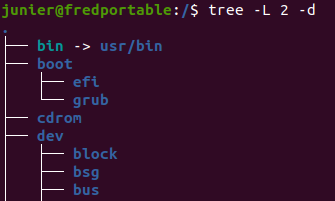
\includegraphics[width=0.35\textwidth,height=\textheight]{https://gitlab.com/frederic-junier/nsi-public/-/raw/master/Premiere/Systeme/images/tree-racine.png}
\caption{arborescence racine}
\end{figure}

\begin{enumerate}
\def\labelenumi{\arabic{enumi}.}
\setcounter{enumi}{1}
\item
  La commande \texttt{pwd} pour \texttt{print\ work\ directory} permet
  d'afficher le \emph{répertoire courant dit de travail}. Le symbole
  tilde \texttt{\textasciitilde{}} est un raccourci pour désigner le
  répertoire personnel de l'utilisateur, en général
  \texttt{/home/utilisateur}.

\begin{verbatim}
 junier@fredportable:~/sandbox$ pwd
 /home/junier/sandbox
\end{verbatim}
\item
  La commande \texttt{tree} sans argument permet alors d'afficher toute
  l'arborescence depuis le répertoire courant qui est représenté par un
  \texttt{.}. Le \emph{chemin relatif} du fichier \texttt{photo1.jpg}
  par rapport au répertoire courant \texttt{sandbox} est
  \texttt{./rep1/photo1.jpg} ou \texttt{rep1/photo1.jpg} et son chemin
  absolu par rapport au répertoire racine s'obtient en le faisant
  précéder par le chemin absolu de \texttt{sandbox}, c'est donc
  \texttt{/home/junier/sandbox/rep1/photo1.jpg}.
\end{enumerate}

\begin{figure}
\centering
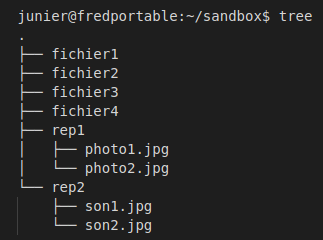
\includegraphics[width=0.35\textwidth,height=\textheight]{https://gitlab.com/frederic-junier/nsi-public/-/raw/master/Premiere/Systeme/images/tree-sandbox.png}
\caption{arborescence relative}
\end{figure}

\begin{enumerate}
\def\labelenumi{\arabic{enumi}.}
\setcounter{enumi}{3}
\item
  La commande \texttt{cd} pour \texttt{change\ directory} permet de
  changer de répertoire courant.

  \begin{itemize}
  \item
    Sans argument ou avec \texttt{cd\ \textasciitilde{}} elle ramène
    l'utlisateur dans son répertoire personnel
    \texttt{/home/utilisateur}. \texttt{cd\ -} ramène dans le répertoire
    précédent

\begin{verbatim}
      junier@fredportable:~/sandbox$ cd
      junier@fredportable:~$ pwd
      /home/junier
      junier@fredportable:~$ cd -
      /home/junier/sandbox
\end{verbatim}
  \item
    \texttt{cd\ ..} permet de remonter dans le répertoire parent :

\begin{verbatim}
     junier@fredportable:~/sandbox$ pwd
     /home/junier/sandbox
     junier@fredportable:~/sandbox$ cd ..
     junier@fredportable:~$ pwd
     /home/junier
\end{verbatim}
  \item
    On peut fournir à \texttt{cd} un chemin absolu ou relatif mais il
    faut que le chemin soit uniquement constitué de répertoires !

\begin{verbatim}
      junier@fredportable:~/sandbox$ cd /home/junier/sandbox/rep1
      junier@fredportable:~/sandbox/rep1$ cd ..
      junier@fredportable:~/sandbox$ cd rep1
      junier@fredportable:~/sandbox/rep1$ cd photo1.jpg
      bash: cd: photo1.jpg: N'est pas un dossier  
\end{verbatim}
  \end{itemize}
\end{enumerate}

\hypertarget{copier-supprimer-duxe9placer-un-fichier}{%
\section{Copier, supprimer, déplacer un
fichier}\label{copier-supprimer-duxe9placer-un-fichier}}

\begin{enumerate}
\def\labelenumi{\arabic{enumi}.}
\item
  La commande \texttt{mv} pour \texttt{move} sert à déplacer ou renommer
  des fichiers ou des répertoires. Elle prend deux arguments
  \emph{source} et \emph{cible} : si la \emph{cible} est un répertoire,
  alors la \emph{cible} est copiée dedans sinon elle est renommée.

\begin{verbatim}
 junier@fredportable:~/sandbox$ ls
 fichier1  fichier2  fichier3  fichier4  rep1  rep2  rep3
 junier@fredportable:~/sandbox$ mv fichier1 fichier1-copie
 junier@fredportable:~/sandbox$ ls
 fichier1-copie  fichier2  fichier3  fichier4  rep1  rep2  rep3
 junier@fredportable:~/sandbox$ ls rep1
 photo1.jpg  photo2.jpg
 junier@fredportable:~/sandbox$ mv fichier1-copie rep1
 junier@fredportable:~/sandbox$ ls rep1
 fichier1-copie  photo1.jpg  photo2.jpg
 junier@fredportable:~/sandbox$ mv rep1 rep2
 junier@fredportable:~/sandbox$ ls rep2
 rep1  son1.jpg  son2.jpg
\end{verbatim}
\item
  La commande \texttt{cp} permet de copier des fichiers. Elle s'utilise
  comme \texttt{mv}, sauf que le fichier \emph{source} n'est pas
  supprimé. Par défaut \texttt{cp} ne copie que des fichiers, pour
  copier un répertoire et son contenu, il faut lui passer l'option
  \texttt{-R} pour \texttt{recursive}.

\begin{verbatim}
 junier@fredportable:~/sandbox$ ls
 fichier2  fichier3  fichier4  rep2  rep3
 junier@fredportable:~/sandbox$ ls rep2
 rep1  son1.jpg  son2.jpg
 junier@fredportable:~/sandbox$ cp fichier2 rep2
  junier@fredportable:~/sandbox$ ls rep2
 fichier2  rep1  son1.jpg  son2.jpg
 junier@fredportable:~/sandbox$ cp rep2 rep3
 cp: -r non spécifié ; omission du répertoire 'rep2'
 junier@fredportable:~/sandbox$ cp -R rep2 rep3
 junier@fredportable:~/sandbox$ ls rep3
 rep2
\end{verbatim}
\item
  La commande \texttt{rm} permet de supprimer les fichiers qu'on lui
  passe en argument. Pour supprimer un répertoire et son contenu, il
  faut lui passer l'option \texttt{-R} comme pour \texttt{cp}.
  \emph{Attention, \texttt{rm} ne déplace pas les fichiers vers une
  corbeille, ils sont supprimés définitivement !}

\begin{verbatim}
 junier@fredportable:~/sandbox$ ls
 fichier2  fichier3  fichier4  rep2  rep3
 junier@fredportable:~/sandbox$ rm fichier2
 junier@fredportable:~/sandbox$ ls
 fichier3  fichier4  rep2  rep3
 junier@fredportable:~/sandbox$ rm rep3
 rm: impossible de supprimer 'rep3': est un dossier
 junier@fredportable:~/sandbox$ rm -r rep3
 junier@fredportable:~/sandbox$ ls
 fichier2  fichier3  fichier4  rep2
\end{verbatim}
\end{enumerate}

\hypertarget{expansion-des-noms-de-fichiers-et-globbing}{%
\section{\texorpdfstring{Expansion des noms de fichiers et
\emph{globbing}}{Expansion des noms de fichiers et globbing}}\label{expansion-des-noms-de-fichiers-et-globbing}}

On peut agir en masse sur des fichiers grace aux mécanismes d'expansion
de la ligne de commandes : certains caractères spéciaux indiquent au
\emph{shell} qu'il peut les remplacer par des ensembles de caractères.
On peut ainsi décrire des motifs (ou \emph{pattern}) pour décrire des
ensembles de noms de fichiers.

Pour les exemples, on considère un répertoire \texttt{rep3} qui contient
plusieurs fichiers :

\begin{verbatim}
    junier@fredportable:~/sandbox/rep3$ ls
    image1.jpeg  image1.jpg  image1.png  image2.jpeg  image2.jpg  image2.png  image3.jpeg  image3.jpg  image3.png  image4.jpeg
\end{verbatim}

\begin{itemize}
\item
  Le caractère spécial \texttt{*} représente n'importe quelle suite de
  caractères. Par exemple pour lister les fichiers dont le nom de base
  se termine par 1 et l'extension par \texttt{g} on peut écrire :

\begin{verbatim}
       junier@fredportable:~/sandbox/rep3$ ls *1.*g
       image1.jpeg  image1.jpg  image1.png
\end{verbatim}
\item
  Le caractère spécial \texttt{?} représente un caractère unique
  quelconque. Par exemple pour lister les fichiers dont le nom de base
  se termine par 1 et l'extension comporte trois caractères et se
  termine par \texttt{g} on peut écrire :

\begin{verbatim}
       junier@fredportable:~/sandbox/rep3$ ls *1.??g
       image1.jpg  image1.png
\end{verbatim}
\item
  Dans un nom de fichier existant\texttt{\{a..z\}} représente un
  caractère entre \texttt{a} et \texttt{z}. Par exemple pour lister les
  fichiers \texttt{image1.png}, \texttt{image2.png} et
  \texttt{image3.png} on peut écrire :

\begin{verbatim}
        junier@fredportable:~/sandbox/rep3$ ls image{1..3}.png
        image1.png  image2.png  image3.png
\end{verbatim}
\end{itemize}

\hypertarget{gestion-des-droits-sur-les-fichiers}{%
\section{Gestion des droits sur les
fichiers}\label{gestion-des-droits-sur-les-fichiers}}

Considérons le contenu du répertoire \texttt{\textasciitilde{}/sandbox}
affiché de façon détaillée avec la commande \texttt{ls\ -l} :

\begin{verbatim}
    junier@fredportable:~/sandbox$ ls -l
    total 8
    -rwxrw-r-- 1 junier junier    0 août  16 21:43 fichier3
    -rw-rw-r-- 1 junier junier    0 août  16 21:43 fichier4
    drwxrwxr-x 3 junier junier 4096 août  16 23:29 rep2
    drwxrwxr-x 2 junier junier 4096 août  16 23:33 rep3
\end{verbatim}

\begin{enumerate}
\def\labelenumi{\arabic{enumi}.}
\item
  Les 10 premiers caractère d'une ligne représentent les droits sur le
  fichier (ou le répertoire) :

  \begin{itemize}
  \tightlist
  \item
    Pour \texttt{fichier3} on a \texttt{-rw-rw-r-\/-} :

    \begin{itemize}
    \tightlist
    \item
      le premier caractère \texttt{-} indique qu'il s'agit d'un fichier
    \item
      le premier bloc de trois caractères \texttt{rwx} représente les
      droits pour le \emph{propriétaire (u)} du fichier : \emph{lecture
      (r)}, \emph{écriture (w)} et \emph{exécution (x)}.
    \item
      le second bloc de trois caractères \texttt{rw-} représente les
      droits pour le \emph{groupe (g)} du fichier : \emph{lecture (r)},
      \emph{écriture (w)} et un tiret \texttt{-} qui marque l'absence de
      droit d'exécution
    \item
      le dernier bloc de trois caractères \texttt{rw-} représente les
      droits pour les \emph{autres (o)} utilisateurs du fichier : ce
      sont les mêmes que pour le \emph{groupe}.
    \end{itemize}
  \item
    Pour \texttt{rep2} on a \texttt{drwxrwxr-x} :

    \begin{itemize}
    \tightlist
    \item
      le premier caractère \texttt{d} indique qu'il s'agit d'un
      répertoire
    \item
      les trois blocs de trois caractères suivants énumèrent les droits
      en \emph{lecture (r)}, \emph{écriture (w)}, \emph{exécution (x)}
      des trois types d'utilisateurs du répertoire :
      \emph{propriétaire}, \emph{groupe} et \emph{autres}.
    \end{itemize}
  \end{itemize}
\item
  Le propriétaire d'un fichier ou le superutilisateur \texttt{root} peut
  changer les droits d'un fichier ou d'un répertoire avec la commande
  \texttt{chmod} dont la syntaxe est :

\begin{verbatim}
 chmod [-R] [ugoa][+-=][rwx] fichier
\end{verbatim}

  \begin{itemize}
  \tightlist
  \item
    Les options entre crochets désignent :

    \begin{itemize}
    \tightlist
    \item
      \texttt{u} : le propriétaire
    \item
      \texttt{g} : le groupe
    \item
      \texttt{o} : les autres utilisateurs
    \item
      \texttt{a} : tous les utilisateurs
    \item
      \texttt{+} : ajouter le(s) droit(s)
    \item
      \texttt{-} : enlever le(s) droit(s)
    \item
      \texttt{=} : positionner le(s) droit(s)
    \item
      \texttt{r} : droit de lecture
    \item
      \texttt{w} : droit d'écriture
    \item
      \texttt{x} : droit d'exécution
    \item
      \texttt{-R} : récursivement (nécessaire pour agir sur un
      répertoire)
    \end{itemize}
  \item
    Quelques exemples :

    \begin{itemize}
    \item
      Fixer les droits à -x (écriture seule) pour tous les utilisateurs
      sur \texttt{fichier3} :

\begin{verbatim}
    junier@fredportable:~/sandbox$ chmod a=x fichier3
\end{verbatim}
    \item
      Donner le droit d'écriture aux autres utilisateurs sur
      \texttt{fichier4}:

\begin{verbatim}
    junier@fredportable:~/sandbox$ chmod o+w fichier4
\end{verbatim}
    \item
      Enlever le droit de lecture à tous les utilisateurs sur
      \texttt{fichier4} :

\begin{verbatim}
    junier@fredportable:~/sandbox$ chmod ugo-r fichier4
\end{verbatim}
    \item
      Enlever le droit de lecture au groupe sur le répertoire
      \texttt{rep2} :

\begin{verbatim}
    junier@fredportable:~/sandbox$ chmod -R g-w rep2
\end{verbatim}
    \item
      Affichage des droits après les modifications précédentes :

\begin{verbatim}
    junier@fredportable:~/sandbox$ ls -l
    total 8
    ---x--x--x 1 junier junier    0 août  16 21:43 fichier3
    --w--w--w- 1 junier junier    0 août  16 21:43 fichier4
    drwxrwxr-x 3 junier junier 4096 août  16 23:29 rep2
    drwxrwxr-x 2 junier junier 4096 août  16 23:33 rep3
\end{verbatim}
    \end{itemize}
  \end{itemize}
\item
  Le superutilisateur \texttt{root} peut modifier le propriétaire d'un
  fichier avec la commande \texttt{chown}. Il faut passer l'option
  \texttt{-R} pour modifier le propriétaire d'un répertoire.

\begin{verbatim}
 junier@fredportable:~/sandbox$ sudo chown root fichier3
 [sudo] Mot de passe de junier : 
 junier@fredportable:~/sandbox$ ls -l fichier3
 ---x--x--x 1 root   junier    0 août  16 21:43 fichier3
\end{verbatim}
\item
  Le superutilisateur \texttt{root} peut modifier le groupe d'un fichier
  avec la commande \texttt{chgrp}. Il faut passer l'option \texttt{-R}
  pour modifier le groupe d'un répertoire.

\begin{verbatim}
 junier@fredportable:~/sandbox$ sudo chgrp root fichier3
 junier@fredportable:~/sandbox$ ls -l fichier3
 ---x--x--x 1 root   root      0 août  16 21:43 fichier3
\end{verbatim}
\end{enumerate}

\end{document}
